\setcounter{page}{3}
\chapter{Теоретическая часть}
\section{Элементы языка: определение, синтаксис, представление в памяти.}
Элементами языка Lisp являются атомы и структуры (такие как список и точечная пара). Вся информация (данные и программы) в Lisp представляется в виде символьных выражений~---~S-выражений. 
\begin{equation}
	S-\text{выражение} ::= <\text{атом}> | <\text{точечная пара}>.
\end{equation}

Атомы:
\begin{itemize}
	\item символы (идентификаторы)~---~синтаксически~---~набор литер (букв и цифр), начинающихся с буквы;
	\item специальные символы~---~Т, NIL (используются для обозначения логических констант);
	\item самоопределимые атомы~---~натуральные числа, дробные числа (например 2/3), вещественные числа, строки~---~последовательность символов, заключенных в двойные апострофы (например “abc”).
\end{itemize}

%В памяти атомы представлены по разному.
%
%Символы представлены в памяти пятью указателями.
%\begin{itemize}
%	\item name~---~имя (например, A);
%	\item value~---~значение (например, 1);
%	\item function~---~лямбда-выражение;
%	\item properties~---~список свойств;
%	\item package~---~пакет, указатель на начало области; пространство имен;
%\end{itemize}
%
%Благодаря такой организации символ может означать и значение и функцию.
 
Самоопределимые атомы нельзя переопределить или создать функцию с именем самоопределимого атома. Специальные символы нельзя переопределить, но можно создать функцию с именем NIL. Символам можно присваивать значение переменной и функции.

Структуры строятся из бинарных узлов.
Структуры:
\begin{eqnarray}
	\text{точечная пара} ::= (<\text{атом}>.<\text{атом}>) | (<\text{атом}>.<\text{точечная пара}>)\nonumber\\ |
(<\text{точечная пара}>.<\text{атом}>) | (<\text{точечная пара}>.<\text{точечная пара}>),
\end{eqnarray}

\begin{equation}
\text{список} ::= <\text{пустой список}> | <\text{непустой список}>, где 
\end{equation}

\begin{equation}
<\text{пустой список}> ::= ( ) | Nil,\\	
\end{equation}

\begin{equation}
<\text{непустой список}>::= (<\text{первый элемент}> . <\text{хвост}>), \\
\end{equation}

\begin{equation}
<\text{первый элемент}> ::= <\text{S-выражение}>,\\
\end{equation}

\begin{equation}
<\text{хвост}> ::= <\text{список}>.
\end{equation}

Точечная пара является более общей структурой чем список (список является частным случаем точечной пары). Любая непустая структура Lisp в памяти представляется списковой ячейкой, хранящей два указателя: на голову (первый элемент) и хвост~---~все остальное.

\begin{table}[h!]
  \centering
  \begin{tabular}{p{1\linewidth}}
    \centering
    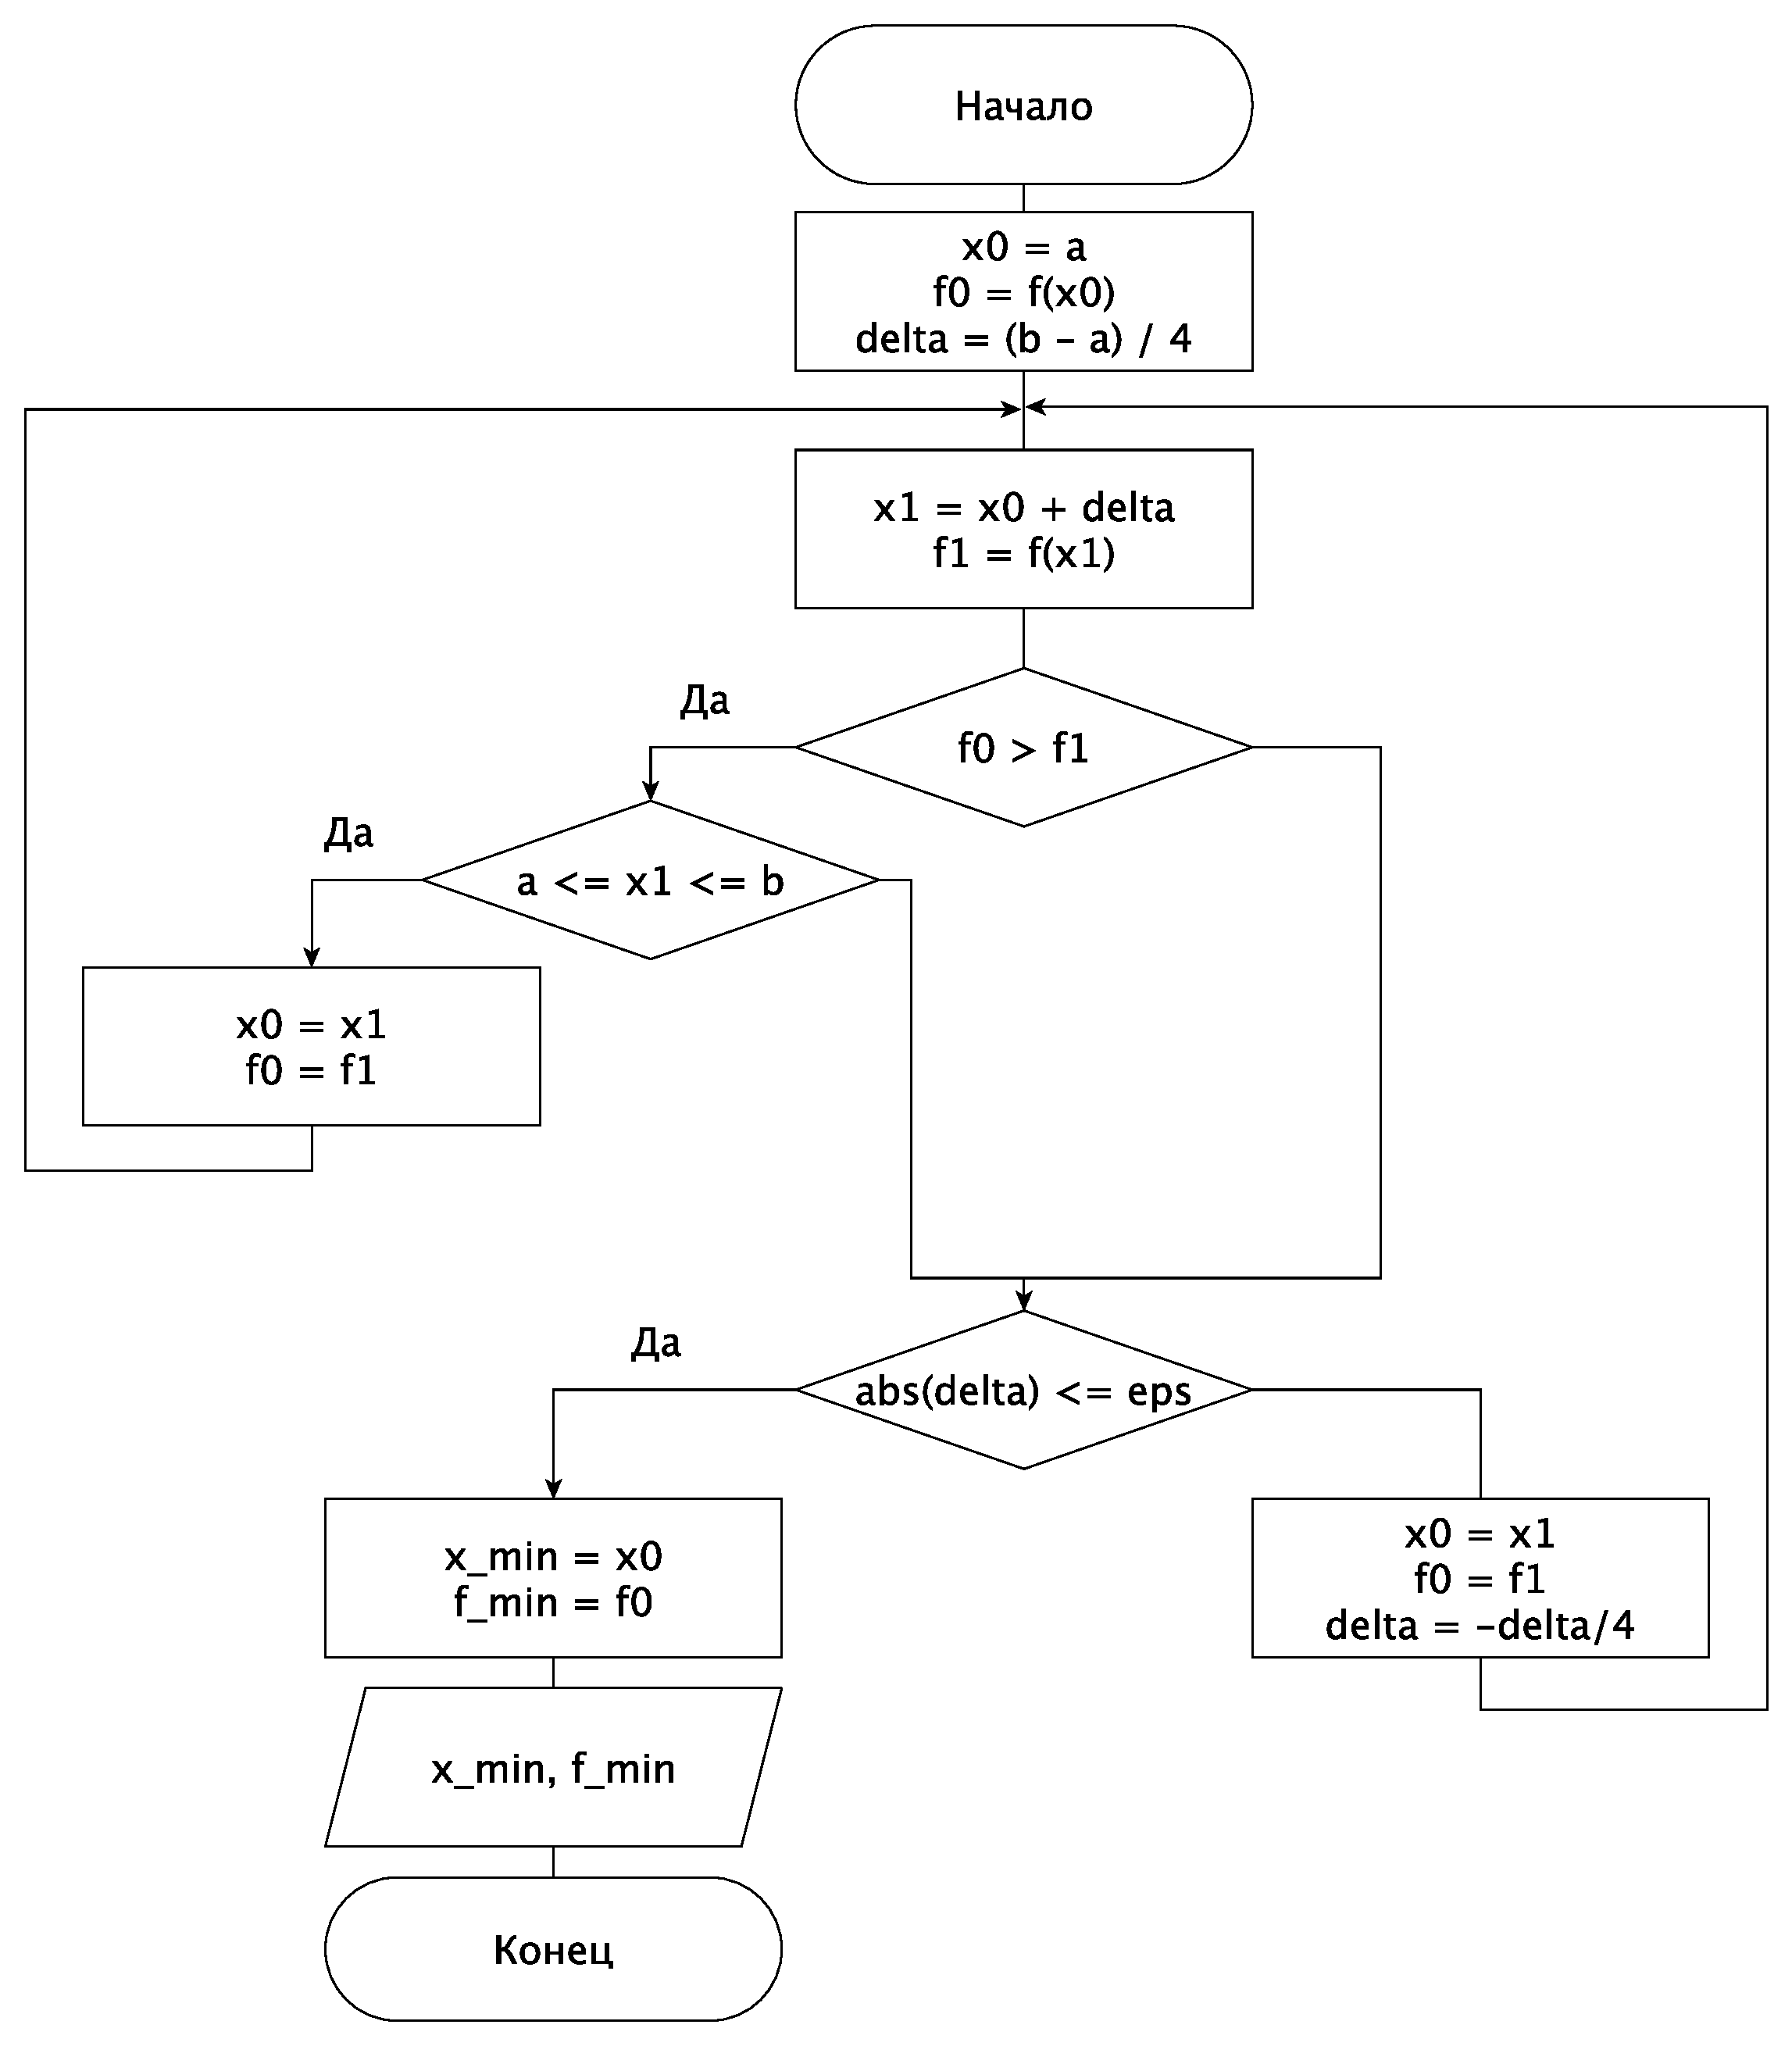
\includegraphics[width=0.4\linewidth]{./images/1.pdf}
    \captionof{figure}{Бинарный узел}
    \label{img:1}
  \end{tabular}
\end{table}

Синтаксис:
\begin{itemize}
	\item любая структура заключается в круглые скобки (A . B)~---~точечная пара, (А)~---~список из одного элемента, пустой список изображается как Nil или ( );
	\item непустой список по определению может быть изображен как (A . (B .  (C . (D ())))), допустимо изображение списка последовательностью атомов, разделенных пробелами~---~(A B C D);
	\item элементы списка могут, в свою очередь, быть списками, например~---~(A (B C) (D (E))).
\end{itemize}

Таким образом, синтаксически наличие скобок является признаком структуры~---~списка или точечной пары.

Точечная пара~---~это пара атомов или точечных пар или их комбинация.

Список~---~это структура данных. Может быть пустой и непустой. Если непустой, то состоит из двух элементов: первый (голова)~---~любая структура (нет слова тип), а второй (хвост)~---~список. По умолчанию первый аргумент списка~---~имя функции, остальные~---~аргументы функции.

\begin{table}[h!]
  \centering
  \begin{tabular}{p{1\linewidth}}
    \centering
    \includegraphics[width=0.35\linewidth]{./images/5.pdf}
    \captionof{figure}{Множества элементов языка}
    \label{img:1}
  \end{tabular}
\end{table}

\section{Особенности языка Lisp. Структура программы. Символ апостроф.}
Программы, написанные на Lisp, представляются в виде его же структур данных, то есть синтаксического отличия нет. Таким образом, можно выдать программы за данные или наоборот, то есть программа способна менять сама себя. Программа на языке Lisp представляет собой последовательность вычислимых выражений, которые являются атомами или списками. Символ ' (апостроф) эквивалентен функции $quote$~---~блокирует вычиcление выражения, и оно воспринимается интерпретатором как данные. Также, Lisp~---~бестиповой язык, поэтому выделяемые под элементы объёмы памяти унифицированы.

\section{Базис языка Lisp. Ядро языка.}
Базис~---~это минимальный набор правил/конструкций языка, к которым могут быть сведены все остальные. Базис языка Lisp представлен атомами, структурами, базовыми функциями, базовыми функционалами. Некоторые базисные функции: $car$, $cdr$, $cons$, $list$, $lambda$, $quote$, $eq$, $eql$, $equal$, $eval$, $apply$, $funcall$. Ядром языка называется базис языка и функции стандартной библиотеки (часто используемые функции, созданные на основе базиса).

Этапы обработки выражения:
\begin{enumerate}
	\item ожидание ввода s-выражения;
	\item передача его функции $eval$, она вычисляет значение переданного аргумента и возвращает его, как результат;
	\item вывод полученного результата.
\end{enumerate}


\newpage

\chapter{Практическая часть}
\section{Задание №1}
Решено на первом занятии. Решение приложено к отчёту.

\section{Задание №2}
Используя только функции CAR и CDR, написать выражения, возвращающие второй, третий, четвертый элементы заданного списка.

CAR принимает точечную пару или список в качестве аргумента и возвращает первый элемент (голову) или NIL, если передан пустой список. CDR принимает точечную пару или список и возвращает хвост. В случае аргумента-непустого списка будет возвращен список, состоящий из всех элементов, кроме первого. В случае аргумента-пустого списка возвращается NIL.

\begin{code}
\caption{Задание №2}
\label{code:bf2}
\begin{minted}{lisp}
; Получить i-ый элемент списка
(CAR (CDR '(1 2 3 4))) ; 2-ой
(CAR (CDR (CDR '(1 2 3 4)))) ; 3-ий
(CAR (CDR (CDR (CDR '(1 2 3 4))))) ; 4-ый
\end{minted}
\end{code}

\section{Задание №3}
Что будет в результате вычисления выражений? (ответ написан в комментарии после каждого выражения).

Пояснение:
\begin{itemize}
	\item (CAADR ' ((blue cube) (red pyramid))) == (CAR (CAR (CDR '((blue cube) (red pyramid)))))
	\item (CDAR '((abc) (def) (ghi))) == (CDR (CAR '((abc) (def) (ghi))))
	\item (CADR '((abc) (def) (ghi))) == (CAR (CDR '((abc) (def) (ghi))))
	\item (CADDR '((abc) (def) (ghi))) == (CAR (CDR (CDR '((abc) (def) (ghi)))))
\end{itemize}

\begin{code}
\caption{Задание №3}
\label{code:bf3}
\begin{minted}{lisp}
(CAADR '((blue cube) (red pyramid))) ; RED
(CDAR '((abc) (def) (ghi))) ; NIL
(CADR '((abc) (def) (ghi))) ; (DEF)
(CADDR '((abc) (def) (ghi))) ; (GHI)
\end{minted}
\end{code}

\section{Задание №4}
Напишите результат вычисления выражений (ответ написан в комментарии после каждого выражения).

Пояснение:
\begin{itemize}
	\item Функция $list$ возвращает список, содержащий значения переданных ей аргументов. Элемент с апострофом интерпретатор воспринимает как данные. 
	\item Функция $cons$ создает списковую ячейку с первым аргументом-головой и вторым-хвостом. Первый аргумент $cons$ может быть любым из допустимых в языке, а второй обязательно список. Если второй аргумент является атомом, то создаётся точечная пара. Если второй аргумент является списком, то возвращается список, объединяющий предыдущие элементы с элементами второго аргумента-списка.
\end{itemize}

\begin{code}
\caption{Задание №4}
\label{code:bf4}
\begin{minted}{lisp}
(list 'Fred 'and 'Wilma) (list 'Fred '(and Wilma)) (cons Nil Nil) 
; (FRED AND WILMA) (FRED (AND WILMA)) (NIL)

(cons T Nil) ; (T)

(cons Nil T) ; (NIL . T)

(list Nil) ; (NIL)

(cons ' (T) Nil) ; ((T))
\end{minted}
\end{code}

\newpage

\begin{code}
\caption{Задание №4}
\label{code:bf44}
\begin{minted}{lisp}
(list ' (one two) ' (free temp)) ; ((ONE TWO) (FREE TEMP))
(cons 'Fred '(and Wilma)) (cons 'Fred '(Wilma)) (list Nil Nil) 
; (FRED AND WILMA) (FRED WILMA) (NIL NIL)

(list T Nil) ; (T NIL)

(list Nil T) ; (NIL T)

(cons T (list Nil)) ; (T NIL) 

(list '(T) Nil) ; ((T) NIL)

(cons '(one two) '(free temp)) ; ((ONE TWO) FREE TEMP)
\end{minted}
\end{code}

\section{Задание №5}
Написать лямбда-выражение и соответствующую функцию:
Написать функцию (f arl ar2 ar3 ar4), возвращающую список: ((arl ar2) (ar3 ar4)).
Написать функцию (f arl ar2), возвращающую ((arl) (ar2)).
Написать функцию (f arl), возвращающую (((arl))). Представить результаты в виде списочных ячеек.

Функция~---~однозначное отображение множества значений аргументов в значение функции. Базисные функции~---~предоставляются языком, минимально необходимые для работы языка.

По аргументам и поведению:
\begin{itemize}
	\item Базовые/чистые функции~---~фиксированное количество аргументов, для определенного набора аргументов один фиксированный результат;
	\item Формы~---~функции, которые принимают произвольное количество аргументов или по разному обрабатывают аргументы;
	\item Функционалы (высшего порядка)~---~в качестве аргумента принимают функцию или возвращают функцию.
\end{itemize}

По именованию:
\begin{itemize}
	\item Именованные~---~имеют имя, можно определить через defun. Специальные символы (T, NIL) и самоопределимые атомы (натуральные, вещественные числа, строки) не могут выступать в роли функции;
	\item Неименованные~---~нет имени, определяются с помощью $lambda$.
\end{itemize}

\begin{code}
\caption{Задание №5}
\label{code:bf5}
\begin{minted}{lisp}
; Задание: (f arl ar2 ar3 ar4) => ((arl ar2) (ar3 ar4))
; лямбда-выражение
((lambda (ar1 ar2 ar3 ar4) (list (list ar1 ar2) (list ar3 ar4))) 1 2 3 4)
; функция
(defun f1 (ar1 ar2 ar3 ar4) (list (list ar1 ar2) (list ar3 ar4)))
; вызов функции
(f1 1 2 3 4)
\end{minted}
\end{code}

\begin{table}[h!]
  \centering
  \begin{tabular}{p{1\linewidth}}
    \centering
    \includegraphics[width=1\linewidth]{./images/2.pdf}
    \captionof{figure}{Результат 1}
    \label{img:2}
  \end{tabular}
\end{table}

\begin{code}
\caption{Задание №5}
\label{code:bf55}
\begin{minted}{lisp}
; Задание: (f arl ar2) => ((arl) (ar2))
; лямбда-выражение
((lambda (ar1 ar2) (list (list ar1) (list ar2))) 1 2)
; функция
(defun f2 (ar1 ar2) (list (list ar1) (list ar2)))
; вызов функции
(f2 1 2)
\end{minted}
\end{code}

\begin{table}[h!]
  \centering
  \begin{tabular}{p{1\linewidth}}
    \centering
    \includegraphics[width=1\linewidth]{./images/3.pdf}
    \captionof{figure}{Результат 2}
    \label{img:3}
  \end{tabular}
\end{table}

\begin{code}
\caption{Задание №5}
\label{code:bf555}
\begin{minted}{lisp}
; Задание: (f arl) => (((arl)))
; лямбда-выражение
((lambda (ar1) (list (list (list ar1)))) 1)
; функция
(defun f3 (ar1) (list (list (list ar1))))
; вызов функции
(f3 1)
\end{minted}
\end{code}

\begin{table}[h!]
  \centering
  \begin{tabular}{p{1\linewidth}}
    \centering
    \includegraphics[width=0.4\linewidth]{./images/4.pdf}
    \captionof{figure}{Результат 3}
    \label{img:4}
  \end{tabular}
\end{table}

\newpage